\documentclass{../../../lessonplan}
\renewcommand{\cflroot}{../../..}

\begin{document}

\lessonplantitle
    {KS1-S5}
    {Key Stage 1 Session 7}
    {Introducing the repeat code}

\preamble
    {
    \item Understand and use simple repetition
    }
    {
    \item Levels 19 to 22 in Rapid Router
    \item Video 3
    \item Screen shots of levels 20 to 22 from the Levels Guide
    \item Resource sheets KS1-S7-1 to KS1-S7-3
    \item Interactive Whiteboard (IWB)
    }
    {
    \item Repeat, repetition
    }

\begin{lessonplan}

Show \textbf{Video 3} to introduce the idea of a \keyword{repeat} function, which demonstrates how this is important in programming in the wider world \textit{[fig S7.1]}.

\fig{fig S7.1}{figS7.1.jpg}{1}

Bring the children together and show them level 19 \textit{[fig S7.2]}, where a \keyword{repeat} command would be useful.

\fig{fig S7.2}{figS7.2.jpg}{1}

Ask them to write out the instructions they would use to have the least amount of code possible.

Go through the process together on the IWB.

\keyquestion{Can you see a pattern in the instructions?}

Discuss what they see.
If we explained this in English we might use words like `over again'.

Explain that programming languages have a word for this: \keyword{repeat}.

Introduce the \keyword{repeat} command in the app.

\begin{center}
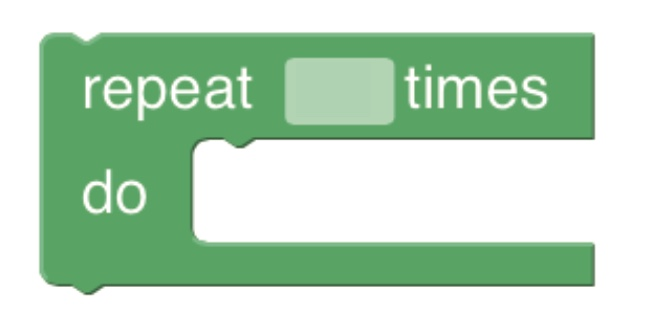
\includegraphics[width=.667\linewidth]{repeat.jpg}
\end{center}

Demonstrate how to use this by dragging it across, clicking on the number to choose the times to repeat, and dragging the move blocks in into the repeat loop.

Look at level 20 \textit{[fig S7.3]}, and go through the process of showing the code step-by-step, seeing the pattern and shortening the code to a repeat loop.

\fig{fig S7.3}{figS7.3.jpg}{1}

\section*{Unplugged activity}

Talk about what things we repeat in other areas of learning.

Start a clapping rhythm and ask the children to repeat it three times.
Think of some poems where lines are repeated.

\section*{Independent activity}

Most children will be ready to refine their programs by using the repeat loops in levels 19-21.
Some may go on to try level 22, which is covered in session 8.
For levels 20-21, some children will benefit from building the code step-by-step.
Spotting the pattern, separating out the set of instructions to be repeated using the repeat block around that set, and placing the superfluous code in the workspace bin.
Have printed copies of levels 20-21 for the children to mark repeated sections.

\subsection*{Support}

Some children may need to walk though the repeat sequence.
You can do this by making a repeat pattern path on the floor with masking tape, and asking the children to work out the algorithm using \keyword{forward} and \keyword{turn} instructions.

\subsection*{Share and review}

Discuss what they have learnt.

\keyword{Can you explain why it is useful to have a block for \keyword{repeat}?}

Look at level 22 \textit{fig S7.4} together.
If any children have tackled this, ask them to explain to the class how they approached it, and say that you will start with this next lesson.

\fig{fig S7.4}{figS7.4.jpg}{1}

Recap on the programming commands they have learnt so far and add \keyword{repeat} to you code wall display.
Use resource sheets KS1-S7-1 to KS1-S7-3 for homework / consolidation.

\end{lessonplan}

\end{document}
